\section{Completed experiments and what they establish}
\label{sec:evidence}

\subsection{Evidence design}

The package retains exact sources, positive certificates, source reconstruction
records, independent finite oracles, raw timing rounds, and explicit negative
controls. Its tests answer different questions: local algebraic completeness
on specified finite sources, preservation of a complete marked signature,
correctness of graph assembly, correctness of the original-source witness,
and native geometric coverage. Their counts should not be added and described
as distinct knot instances.

The final quick runner executes 27 routing/reblocking test methods, 14 bundle
test methods, and 11 cancellation test methods, then replays the retained
graph and native positive certificates. These are focused suites for the
additive prototypes. The maintained recognizer's full regression suite and
end-to-end native knot benchmarks are outside the reported experiment.

\subsection{Implementation and finite evidence for profile discovery}
\label{sec:profile-evidence}

The general component-budget search is implemented in
\path{normal_weight_clusters.py}. It enumerates connected supports,
constructs exact local affine profiles, retains admissible positive even
increments, and reuses those profiles in disjoint component products.
It also implements the dependent-baseline homogeneous exception.
Projected rows are deduplicated, and a same-sign test rejects equations
that cannot have strictly positive increments.  All source conditions
are checked.  The component budget is capped at $\min(r,k)$, including
when the supplied integer $r$ is very large.  Global work, support,
linear-system, and product limits remain effective through final
certificate replay; a limit reports incomplete search.

The supplied vertex gate is an unchanged copy of the incoming
rank-and-boundary checker.  It verifies a primitive supported normal
ray, Euler characteristic one, and essential boundary through exact
linear algebra and boundary cohomology.  Positive results are replayed
by the separate checker.  Exhaustion concerns only the stated source
and parameter class and yields no unrestricted knot verdict.  The
overlay leaves the maintained recognizer and its defaults unchanged.

\subsubsection{Complete radius-two candidate generation}

The paired experiment compares the new profile search with the incoming
enumerator over all supports of size at most two.  Each timed call
includes source and cocycle preparation, complete candidate generation,
local normal reconstruction, and actual-cancellation filtering; neither
arm includes a topological vertex-disc gate.  Candidate sets are checked
for exact equality outside the timed blocks.  Each source receives one
excluded warmup per arm and five measured rounds, with arm order
shuffled using a recorded seed.  Table~\ref{tab:profile-radius-two}
reports seconds and ratios of the two arm medians; these are not medians
of per-round ratios.  Full samples, observed ranges, counters, and hashes
are in \texttt{artifacts/benchmark.json}.

\begin{table}[htbp]
\centering
\small
\begin{tabular}{lrrrr}
\hline
Source & $t$ & All supports (s) & Profiles (s) & Ratio\\
\hline
Layered obstruction & 8 & 1.189400 & 0.026278 & $45.26$\\
Layered obstruction & 16 & 7.213136 & 0.043151 & $167.16$\\
Layered obstruction & 24 & 25.963222 & 0.060250 & $430.93$\\
Layered obstruction & 40 & 122.938084 & 0.096843 & $1269.46$\\
Disconnected-support source & 15 & 4.006094 & 0.041128 & $97.40$\\
\hline
\end{tabular}
\caption{Complete radius-two candidate generation, five measured
rounds.  The ratio is the all-support median divided by the profile
median.  Exact resulting candidate sets agree in every case.}
\label{tab:profile-radius-two}
\end{table}

The counts make the change in workload concrete.  At $t=40$, the
incoming arm examines $904$ weight spaces and $156\,927$ small systems;
the profile arm examines $173$ connected supports and $4\,051$ systems.
Only two local profiles survive, producing three assembled candidates
including the coherent candidate.  For the disconnected-support source,
the corresponding counts are $154$ spaces and $14\,942$ systems versus
$78$ connected supports and $1\,420$ systems.  Three reusable local
profiles produce five assembled candidates.  Maximum tetrahedron-edge
incidence is $d=6$ in the smallest layered source and $d=8$ in the other
sources.

These gains combine component reuse, smaller connected-support
enumeration, projected-row deduplication, and the stricter local
positive-even-increment filters.  The old baseline first searches
homogeneous weight spaces and filters the actual cancellation support
after reconstruction.  Thus the table does not isolate connectedness
as the sole cause of the speedup.  The source family is deliberately
structured, the parameter radius is small, and these finite timings
establish neither a corpus-wide speedup nor an asymptotic growth law.

\subsubsection{A retained whole-query regression}

The existing incoming one-edge specialization is a stronger practical
baseline for positive radius-one queries.  A second paired experiment
therefore compares complete successful queries, including internal
positive verification and replay.  Both methods find the same certified
disc on these sources.  Here there is one excluded warmup per arm and
seven measured rounds, again with shuffled arm order.  The incoming
method uses its native component observer, whereas the new method uses
the polynomial rank gate.  Their end-to-end costs consequently include
different verification mechanisms, an intentional part of this
integration comparison.

\begin{table}[htbp]
\centering
\small
\begin{tabular}{rrrr}
\hline
$t$ & Incoming one-edge (s) & Profiles with rank gate (s) & Slowdown\\
\hline
8 & 0.002818 & 0.005381 & $1.91$\\
16 & 0.004930 & 0.014919 & $3.03$\\
24 & 0.007299 & 0.034642 & $4.75$\\
40 & 0.012197 & 0.128793 & $10.56$\\
\hline
\end{tabular}
\caption{Complete positive radius-one queries, seven measured rounds.
The slowdown is the new median divided by the incoming median, not the
median of paired sample ratios.}
\label{tab:profile-radius-one}
\end{table}

The larger-radius search improvement therefore does not justify
replacing the existing one-edge specialization.  A practical portfolio
should retain it, while adding component profiles for larger budgets.
The polynomial bit-complexity guarantee of the rank gate also does not
imply lower constants on these small positive instances.  All measured
regressions are retained in the artifact.

\subsubsection{Validation and evidential limits}

All eleven focused tests pass.  They compare exhaustive candidate sets
on actual sources; recover the disconnected witness through the
independent incoming weight-space enumerator; exercise the homogeneous
exception; compare connected-set enumeration with brute subsets; check
global resource limits, external cancellation, and input immutability;
replay certificates with discovery routines disabled; reject forged
certificates; and exercise exact arithmetic with an $8193$-bit right
hand side.  That last test validates the local arithmetic path, not a
complete topological search at that coordinate size.

The retained fifteen-tetrahedron source includes its full face
pairings, construction history, independently checked Pachner moves,
and positive vertex-disc certificates.  Its independently generated
dense one-edge inventory proves the finite statement
$\kappa_V=2$ as described in
Proposition~\ref{prop:cluster-fixture-minimum}.  The separate full census
contains $821$ standard vertex vectors agreed upon by Regina's direct
tree and direct double-description algorithms; the three meridians all
have two cancellation components.  Each positive is independently
certified.  Completeness of this additional census still relies on
those external enumeration algorithms.  No generic independently
replayable certificate for unrestricted negative assertions is supplied.

The new module, tests, measurement driver, finite-audit scripts, and
theorem fragment form an additive research artifact.  They establish a
proved search guarantee for an explicit source class and measured gains
for complete radius-two candidate generation, together with a concrete
integration regression.  A global quasipolynomial recognizer still
requires the structural and source-coverage results stated elsewhere in
this article.


\subsection{Native coverage and measured costs}

The complete retained source corpus contains 106 normal-cut inputs.  The
previous disk-only classifier certified 30; the new unsaturated classifier
certified 35 and preserved every previous census.  All 35 complete outputs
passed independent source-proof replay.  Each of the five newly covered
inputs was also cut explicitly by Regina 7.4; its component-by-component
\texttt{recogniseHandlebody} results agreed exactly.  The remaining 71 cases
consist of 55 saturated-base cases, 6 raw-cancellation stalls, and 10 cores
with three-handles.  These are inconclusive outcomes, not non-handlebody
verdicts.

\begin{center}
\begin{tabular}{lrrr}
\hline
Case & New+replay (ms) & Explicit Regina (ms) & Old (ms)\\
\hline
LST(5,7) & 51.439 & 3.025 & 20.729\\
Pachner(3,5,1) & 51.711 & 1.215 & 29.976\\
Pachner(5,8,1) & 82.614 & 2.037 & 42.635\\
Pachner(5,8,2) & 208.660 & 2.774 & 96.788\\
LST(3,8), mixed & 310.987 & 1.881 & 160.733\\
Layered 1, one copy & 2.681 & 0.670 & 2.559\\
Layered 4, eight copies & 423.763 & 24.471 & 433.749\\
Layered 8, one copy & 1886.583 & 195.046 & 1779.949\\
\hline
\end{tabular}
\end{center}

The first five old results were \texttt{INCONCLUSIVE}; their times are not
a speed baseline for a completed answer.  All new times include producer
and source verifier, while Regina times include construction of the
explicit cut, component separation, and recognition.  Five paired rounds
were run after a warmup, with shuffled arm order and garbage collection
outside the timers.  The three preserved cases had old/new paired median
ratios $0.942$, $0.997$, and $0.908$.  On these small inputs the native
certificate path is slower than the compiled Regina oracle.  The observed
advance is additional certified coverage; no practical speedup is claimed
for these fixtures.

For the abstract proper-boundary model with an orientable genus
$g=2^{16384}+17$ base, two boundary circles and one attached annulus,
the output is one handlebody of genus $2g$.  It represents the
$2g$ relative one-handles by an exact counter.  The encoded input has
4,321 bytes and the formatted certificate has 25,130 bytes under the
benchmark serialization.  Production and replay together took a median
$0.180$ milliseconds over five rounds.  No explicit band system or
large surface was constructed.  The finite prototype tests include 700
random assembly comparisons, strict type and source-mutation checks,
producer-disabled replay, saturated refusal, nonorientable-base formulas,
and multiplicities exceeding $2^{20000}$.  Fourteen named test methods
passed with the minimal pinned native runtime.  Timing values are
machine-specific; the raw rounds, environment, source corpus hash, and
five replayable new source certificates accompany the code.


\subsection{Complete signatures, exact source maps, and sharp examples}

The main routing audit samples 240 aligned source tiles of widths one through
three, retaining loops and multiple edges. Twenty-seven sources have
components with unequal input and output widths. An independent frontier
coloring oracle evaluates the assembled kernel; the source is evaluated by
exact marked-signature multiplication. The two exponents per source give 480
complete-signature comparisons covering 53,760 table entries, all equal.
The largest kernel in this audit has 154 edges. Another 60 explicit cubic
source verdicts agree with their kernel verdicts.

A separate reviewer audit reconstructs 300 flat chains with shuffled vertex
identifiers, shuffled edge records, reversed tiles, multiple macros, and
exponents extending beyond $10^{20}$. Its producer/checker graph identities
agree. On 120 finite shuffled and reversed cubic chains, every available
negative witness was expanded to the original source: 105 complete colorings,
covering 96,252 actual edge occurrences, reproduce their exact crossing and
anchor addresses. Additional targeted chains combine unstable periods two
and three, including zero quotients and nonempty remainders in both blocks.

The reblocking audit enumerates all through-component partition diagrams of
widths one through five: respectively $1,3,25,339,6721$, or 7,089 in total.
Independent explicit stacking checks alignment by exponent $d$ and verifies
10,656 strict component-count drops before first alignment. The cubic sharp
family in the wrapper tests attains first alignment $m=d$ for $d=2,\ldots,8$.
These finite checks test the implementation and examples; the equivalence
recurrence proves the bound at arbitrary width.

The exact connected-cutoff audit compares 2,048 full signatures on 64 random
connected tiles at thresholds zero through seven, covering 81,920 entries.
It also checks the small-threshold sharp paths and fourteen comb examples at
$k=3,\ldots,16$. An unrestricted independent max-flow calculation gives
minimum cuts $k$ at exponent $k$ and $k+1$ at exponent $k+1$ for the comb
boundary prescription. All checks pass. The general-threshold production
constructor now uses the proved exact cutoff; the certified topological
pattern query remains threshold three.

\begin{figure}[tb]
\centering
\begin{tikzpicture}[scale=.8,vertex/.style={circle,fill=Ink,inner sep=2.4pt},
 every node/.style={font=\small}]
\foreach \y in {0,1,2}{
 \node[vertex] (a\y) at (0,-\y) {};
 \node[vertex] (b\y) at (2,-\y) {};
 \node[vertex] (c\y) at (6,-\y) {};
 \node[vertex] (d\y) at (8,-\y) {};
 \node[vertex] (e\y) at (10,-\y) {};
}
\draw[Accent,very thick] (a0)--(b0) (a1)--(b0);
\draw[BurntOrange,very thick] (a2)--(b1) (a2)--(b2);
\draw[Ink,very thick] (c0)--(d0) (c1)--(d0) (c2)--(d1) (c2)--(d2)
 (d0)--(e0) (d1)--(e0) (d2)--(e1) (d2)--(e2);
\draw[-{Stealth[length=3mm]},gray,thick] (3,-1)--(5,-1);
\node at (1,.65) {$T$: two components};
\node at (8,.65) {$T^{\circ2}$: connected};
\node[align=center] at (1,-3) {Input blocks $\{0,1\},\{2\}$\\
Output blocks $\{0\},\{1,2\}$};
\node at (8,-2.65) {All three layers are actual interface vertices};
\end{tikzpicture}
\caption{A through tile with initially different component partitions.
After two copies the graph is connected and hence aligned. This diagram
illustrates exact reblocking only; it is not a cubic terminal pattern.}
\label{fig:reblocking}
\end{figure}

\subsection{Large binary graph examples}

The aligned star--triangle tile has seven vertices and six edges, interfaces
$L=(0,1,2)$ and $R=(3,4,5)$, and edge list
\[
 (0,6),(4,6),(5,6),(1,2),(2,3),(3,1).
\]
Its star component transports one input port to two output ports; its
triangle component transports the two remaining input ports to one output.
The induced component permutation is a transposition. Its closed $N$-copy
graph has $4N$ vertices and $6N$ edges. At $N=1$ it is $K_4$, supplying a
positive finite graph certificate. At odd large $N$, the routed kernel has
36 vertices and 54 edges. For $N=2^{4096}+1$, the retained proof lifts its
negative query answer without enumerating any missing copies.

The misaligned through example also uses $N=2^{4096}+1$, but needs an
exact reblocking period of two first. It produces a 54-vertex, 81-edge kernel.
Its source and formatted certificate occupy 1,806 and 11,384 bytes,
respectively. A three-edge cut includes an original edge at copy $N-1$,
which tests the nonzero-tail address formula rather than only an early
retained copy. Five source-production-plus-replay samples have median
1.519 milliseconds. This is a local binary-input demonstration; the
prototype has not constructed a corresponding native knot hierarchy.

For an illustration of the avoided global period, use permutation cycles
of lengths
\[
 2,3,5,7,11,13,17,19,23,29,31,37,41,43,47,53,59,61,67,71.
\]
The width is 639 and their global order is
$557940830126698960967415390$. At exponent $2^{2048}+12345$, componentwise
construction writes 132,226 vertices and 131,587 edges in 0.249 seconds in
the retained run. It never writes that global order as a word. This example
uses matching components and has degree two after closure; it tests only
the general graph-kernel construction and makes no cubic terminal verdict.

\subsection{Paired graph-query performance}

Both timed arms construct their graph, answer the same cubic marked-cut
predicate with the same finite certificate engine, and replay a certificate.
The explicit arm expands the entire source. The routed arm constructs the
bounded kernel and additionally replays its source reduction. Parsing,
serialization, sphere and ball validation, and knot recognition are outside
both timers. Each case has a warmup and seven paired rounds with shuffled
arm order; garbage collection occurs outside each timer. The final routing
run followed completion of the other in-session benchmark jobs.

\begin{center}\small
\begin{tabular}{rrrrrr}
\toprule
Copies & Original edges & Kernel edges & Explicit (ms) & Routed (ms) & Paired ratio\\
\midrule
1 & 6 & 6 & 0.108 & 0.208 & 0.53\\
3 & 18 & 18 & 0.059 & 0.241 & 0.25\\
9 & 54 & 54 & 0.103 & 0.380 & 0.27\\
33 & 198 & 54 & 0.268 & 0.395 & 0.66\\
129 & 774 & 54 & 1.023 & 0.363 & 2.86\\
513 & 3,078 & 54 & 4.281 & 0.377 & 11.04\\
2,049 & 12,294 & 54 & 17.616 & 0.421 & 42.97\\
8,193 & 49,158 & 54 & 80.700 & 0.459 & 198.94\\
\bottomrule
\end{tabular}\end{center}


Times are separate medians; ``paired ratio'' is the median of the seven
within-round explicit/routed ratios, so it need not equal the ratio of the
two displayed medians. The identical-explicit A/A control at 129 copies has
paired median ratio 1.009. The one-, three-, nine-, and thirty-three-copy
cases expose genuine reduction overhead. At 8,193 copies, the explicit
median is 80.700 milliseconds and the routed median is 0.459 milliseconds.
The family has a quickly found negative cut at the larger sizes; this is
a complete local graph query, not a worst-case positive-flow benchmark or a
comparison with the fastest possible cubic-connectivity implementation.

For exponent lengths $65,257,1025,4097,16385$ bits, the same aligned
54-edge kernel has retained query-plus-replay medians
$0.293,0.277,0.305,0.414,0.610$ milliseconds. The corresponding compact
JSON certificate sizes are $1768,1960,2728,5800,18088$ bytes under this
benchmark's serialization. Graph size is constant in that experiment;
arithmetic, source binding, and certificate size still depend on exponent
bit length. The source and certificate formatting for the separate through
example is different and should not be compared byte-for-byte as an
algorithmic compression ratio.

\begin{figure}[tb]
\centering
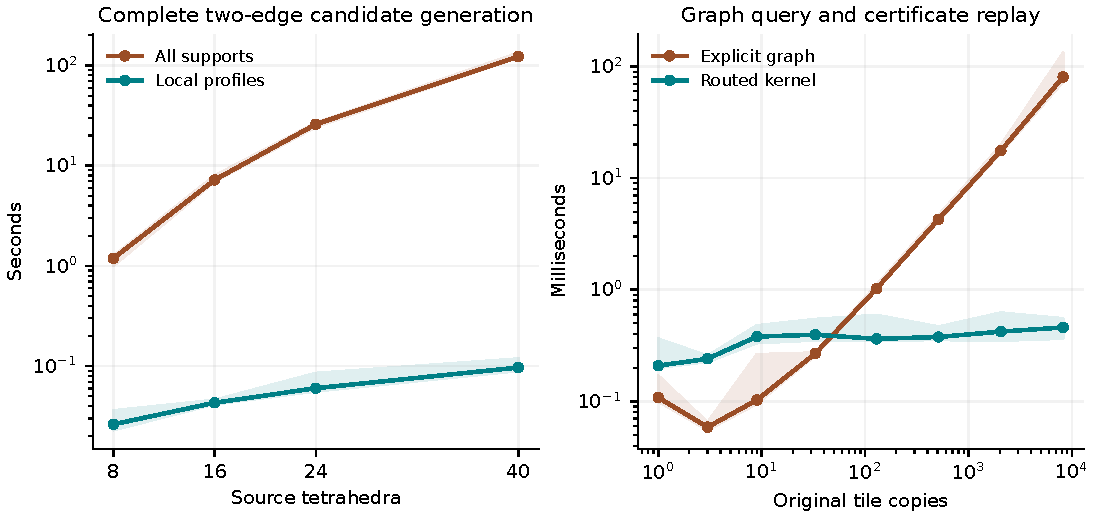
\includegraphics[width=\linewidth]{figures/performance.pdf}
\caption{Two distinct local performance comparisons. Lines show retained
medians and shading shows the observed sample ranges. Left: complete
radius-two candidate generation on the layered obstruction family, with
equal candidate sets and no topology-gate timing. Right: graph construction,
query, and certificate replay on the star--triangle family. These measurements
do not establish an end-to-end asymptotic knot-recognition bound.}
\label{fig:performance}
\end{figure}

\subsection{Interpretation and limitations of the measurements}

The strongest measured search gain is in exhaustive multi-edge candidate
generation. The clearest geometric gain is additional completed native
classifications. The graph gain removes numerical multiplicity from a query
whose faithful source grammar is already supplied. These are different
improvements and cannot be multiplied to obtain a claimed recognition speedup.

All timings come from one shared execution environment and small deliberately
specified families. Raw rounds and ranges are retained; no hardware-isolation
claim is made. The proofs establish the stated asymptotic reductions under
their hypotheses. The experiments establish agreement, rejection behavior,
source lifting, and the local costs actually measured. A broader native
workload is needed to decide the dispatch policy and identify which remaining
geometric interface dominates a complete run.
